\documentclass[12pt]{article}
\usepackage{amsmath}
%----------------------------------------------------------
%информация по ЛР
%----------------------------------------------------------
\newcommand{\Title}{Отчет о выполнении лабораторной работы}
\newcommand{\TaskType}{Лабораторная работа}
\newcommand{\SubTitle}{по дисциплине <<Модели и методы анализа проектных решений>>}
\newcommand{\LabTitle}{Метод конечных элементов} % Указана в задании, можно немного конкретизировать
\newcommand{\VarTitle}{23}
\newcommand{\Faculty}{<<Робототехника и комплексная автоматизация>>}
\newcommand{\Department}{<<Системы автоматизированного проектирования (РК-6)>>}
\newcommand{\AuthorFull}{Шашко Олег Владимирович}
\newcommand{\Author}{Шашко О. В.}
\newcommand{\EduGroup}{РК6-71б}
\newcommand{\Semestr}{осенний семестр} % Например: осенний семестр или весенний семестр
\newcommand{\BeginYear}{2023}
\newcommand{\Year}{2023}
\newcommand{\Country}{Россия}
\newcommand{\City}{Москва}
% Цель выполнения 
\newcommand{\GoalOfResearch}{решение дифференциального уравнения методом конечных элементов (МКЭ), используя линейную и кубическую функции формы, и анализ точности относительной аналитического способа решения } % Цель исследования (с маленькой буквы и без точки на конце)
%----------------------------------------------------------

%----------------------------------------------------------
%общая преамбула для всех лабораторных - настройки общего вида оформления
%----------------------------------------------------------
%\usepackage{mathtext}
\usepackage{amssymb}
\usepackage{amsfonts}
%\usepackage{amsmath}
%\usepackage{mathabx}
\usepackage{MnSymbol}
%\usepackage{stmaryrd}
\usepackage{indentfirst}
\usepackage{graphicx}
\graphicspath{ {./images/} }

\usepackage[T2A]{fontenc}
\usepackage[utf8]{inputenc}
\usepackage[english,russian]{babel} %% это необходимо для включения переносов
\usepackage{float}
\usepackage{rotating}
\usepackage{multirow}
\usepackage{pdflscape}
\usepackage{bm}
% необходимо для возможности копирования и поиска в готовом PDF
\usepackage{cmap} 
\usepackage{array}
\usepackage{multicol}

\usepackage{hyperref}
\hypersetup{colorlinks=true, linkcolor=red}

\usepackage{xspace}

\usepackage{tikz}
\usetikzlibrary{tikzmark}
%\usetikzlibrary{matrix,automata,graphs}
\usetikzlibrary{arrows,positioning,trees}

%----------------------------------------------------------
% необходимо для возможности включать в имена включаемых файлов _
\usepackage[strings]{underscore}
%----------------------------------------------------------
% добавление поддержки команды вывода текста на полях \marginnote
\usepackage{marginnote}
% добавление поддержки команды \color
\usepackage{xcolor}
%--------------------------------------------
% final - удаляет все всплывающие комментарии
\usepackage[author={Alexandr Sokolov},opacity=0.1]{pdfcomment}
%\usepackage[author={Alexandr Sokolov},opacity=0.1,final]{pdfcomment}
\newcommand{\messnote}[1]{\marginnote{\color[rgb]{1,0,0}\Huge\textbf{!}\pdfcomment{#1}}[-1.0cm]}
%----------------------------------------------------------
% Произвольная нумерация списков.
\usepackage{enumerate}
%----------------------------------------------------------
\raggedbottom
%%\hfuzz=10pt
\textwidth=163mm
\textheight=220mm
\oddsidemargin=-0.5pt
\footskip=30pt
\topmargin=27pt
\headheight=12pt
\headsep=25pt
\topskip=10pt
\baselineskip=15pt
\topmargin=-4mm
%----------------------------------------------------------
% указание 
\setcounter{secnumdepth}{2}
%----------------------------------------------------------
% подлкючение пакета для подсчета объектов
\usepackage{totcount}
% регистрируем счетчик страниц
\regtotcounter{page}
%----------------------------------------------------------
% необходимо для работы команды \xspace (умный пробел после замены, осуществляемой некоторой командой в тексте)
\usepackage{xspace}
%----------------------------------------------------------
% определение атрибутов сборки Git
%\usepackage[grumpy, maxdepth=6]{gitinfo2}
%\renewcommand{\gitMark}{\textcolor{gray}{[git] \textbullet{} \gitBranch\,@\,\gitAbbrevHash{} \textbullet{} \gitAuthorName (\gitAuthorIsoDate)}}
%----------------------------------------------------------
% необходимо для того, чтобы в окружениях enumerate можно было менять формат нумерации
\usepackage{enumitem}
%----------------------------------------------------------
%Необходимо для сокращения размера шрифта подписей и сокращения отступов между рисунком и подписью к нему
\usepackage[margin=5pt,font={small, singlespacing}, labelfont={small}, justification=centering, labelsep=period]{caption}
\captionsetup{belowskip=0pt}
%----------------------------------------------------------
\usepackage[numbers]{natbib}
\usepackage{bibentry}
%***natbib, bibentry***%
% Следующий код необходим для того, чтобы исправить конфликт между пакетами natbib+bibentry и стилем оформления ссылок согласно российскому ГОСТу cp1251gost705u
\ifx\undefined\selectlanguageifdefined
\def\selectlanguageifdefined#1{}\else\fi
\ifx\undefined\BibEmph
\def\BibEmph#1{\emph{#1}}\else\fi
%----------------------------------------------------------

% подключение листингов и определение языков
%\usepackage{listingsutf8}
\usepackage{listings}
\usepackage{color}
\definecolor{orange}{rgb}{1, 0.5, 0}
\definecolor{black}{rgb}{0, 0, 0}
\definecolor{gray}{rgb}{0.5, 0.5, 0.5}
\definecolor{blue}{rgb}{0, 0, 1}


\lstset
{
		extendedchars=\true, % включаем не латиницу
%		inputencoding=utf8x,
		frame=tb, % рамка сверху и снизу
		escapechar=|, % |«выпадаем» в LATEX|
		xleftmargin=0.5cm,
		xrightmargin=0.5cm,
		columns=fullflexible,
%		aboveskip=5pt,
		numbers=left,                    % where to put the line-numbers; possible values are (none, left, right)
		numbersep=4pt,                   % how far the line-numbers are from the code
		showspaces=false,
		showstringspaces=false,
		breakatwhitespace=true,         % sets if automatic breaks should only happen at whitespace
		breaklines=true,                 % sets automatic line breaking
		basicstyle=\color{black}\small\sffamily,%\ttfamily,% \sffamily
		commentstyle=\color{gray}\itshape, % шрифт для комментариев
		stringstyle=\color{orange},
%		stringstyle=\bfseries, % шрифт для строк
		numberstyle=\footnotesize\color{gray},
%		numberstyle=\ttfamily\small\color{gray}, % the style that is used for the line-numbers
		keywordstyle=\color{blue}\bfseries,
 %		directivestyle=\color{red},
%		emph={int,char,double,float,unsigned,bool,string},
		emphstyle={\color{blue}\bfseries},
		tabsize=2,
		captionpos=t,
  	morecomment=[l]{\#},
%		otherkeywords={=,==,:,&},
		texcl=true,
}

\lstloadlanguages{Python}

%--------------------------------------------
% необходимо для команды \cancelto{0}{x}
\usepackage{cancel}
%----------------------------------------------------------
% необходимо для того, чтобы доопределить спецификатор P, для 
% использования в таблицах при форматировании
\usepackage{array}
\newcolumntype{P}[1]{>{\centering\arraybackslash}p{#1}}
%----------------------------------------%
% необходимо для того, чтобы допускались разрывы страниц внутри align align*
\allowdisplaybreaks
%----------------------------------------%
%\def\pbs{\raggedright\baselineskip3.0ex}
\def\signhrule{\raggedright\baselineskip30.0ex \vrule height 0.5pt width30mm depth0pt}

\makeatletter
\def\dynscriptsize{\check@mathfonts\fontsize{\sf@size}{\z@}\selectfont}
\makeatother
\def\textunderset#1#2{\leavevmode
  \vtop{\offinterlineskip\halign{%
    \hfil##\hfil\cr\strut#2\cr\noalign{\kern-.3ex}
    \hidewidth\dynscriptsize\strut#1\hidewidth\cr}}}

\newcommand\executer[1]{\textunderset{\scriptsize{подпись, дата}}{\signvrule} #1}
%----------------------------------------------------------
% необходимо для поддержки поворотов текста
\usepackage[absolute]{textpos}
\setlength{\TPHorizModule}{30mm}
\setlength{\TPVertModule}{\TPHorizModule}
\textblockorigin{0mm}{25mm} % start everything near the top-left corner
%----------------------------------------------------------
% оформление "теорем"
\usepackage{amsthm}
%----------------------------------------------------------
\newtheoremstyle{theoremstyle}% <name>
{0pt}% <Space above>
{0pt}% <Space below>
{\normalfont}% <Body font>
{0pt}% <Indent amount>
{\bfseries}% <Theorem head font>
{.}% <Punctuation after theorem head>
{.5em}% <Space after theorem headi>
{}% <Theorem head spec (can be left empty, meaning `normal')>
%----------------------------------------------------------
\theoremstyle{theoremstyle}
%----------------------------------------------------------
%\newtheorem{question}{Вопрос}
%\newtheorem{task}{Задача}
%\newtheorem{solution}{Решение}
\newtheorem{remark}{Замечание}
%----------------------------------------------------------
% атрибуты задачи
\newcommand{\labattributes}[6]{%
\def\tempempty{}
\def\tempa{#1}
\def\tempb{#2}
\def\tempc{#3}
\def\tempd{#4}
  \ifx\tempempty\tempa \def\tempa{доцент кафедры РК-6, кандидат технических наук, доцент, Трудоношин В.А.}\fi
  \ifx\tempempty\tempb \def\tempb{Решение и вёрстка:}\fi
  \ifx\tempempty\tempc \def\tempc{}\fi
  \ifx\tempempty\tempd \def\tempd{}\else \def\tempd{{\textnormal\copyright}~#4}\fi

\vspace{0.5cm}
\begin{flushright}
		\begin{tabular}{p{0.25\textwidth}p{0.7\textwidth}}
		\hfill Постановка: & \copyright~\textit{\tempa} \\
		\hfill \tempb & \copyright~\textit{#5} \\
		\hfill \tempc & \textit{\tempd} \\
		\hfill & \textit{#6}\\
		\end{tabular}
\end{flushright}
}
%----------------------------------------%
% общие определения
\newcommand{\UpperFullOrganisationName}{Министерство науки и высшего образования Российской Федерации}
\newcommand{\ShortOrganisationName}{МГТУ~им.~Н.Э.~Баумана}
\newcommand{\FullOrganisationName}{федеральное государственное бюджетное образовательное учреждение высшего профессионального образования\newline <<Московский государственный технический университет имени Н.Э.~Баумана (национальный исследовательский университет)>> (\ShortOrganisationName)}
\newcommand{\OrganisationAddress}{105005, Россия, Москва, ул.~2-ая Бауманская, д.~5, стр.~1}
%----------------------------------------%
\newcommand{\gitlabdomain}{sa2systems.ru:88}
%----------------------------------------%
\newcommand{\DocOutReference}{\Author. \Title\xspace\SubTitle. [Электронный ресурс] --- \City: \Year. --- \total{page} с. URL:~\url{https://\gitlabdomain} (система контроля версий кафедры РК6)}
%----------------------------------------------------------
% Тематики 
%----------------------------------------------------------
\newcommand{\topicInterpolation}{Интерполяционные многочлены Лагранжа и Эрмита. Численное интегрирование}
\newcommand{\topicDerivation}{Интерполяция сплайнами. Численное дифференцирование}
\newcommand{\topicIntegration}{Автоматическое дифференцирование. Численное интегрирование (квадратуры Гаусса, Гаусса--Лобатто). Ортогональные системы функций. Многочлены Лаггера}
\newcommand{\topicLeastSquareMethod}{Метод наименьших квадратов. Линейная регрессия. Тригонометрическая аппроксимация. Алгоритм Кули--Тьюки. Дискретное преобразование Фурье}
\newcommand{\topicODESolution}{Задача Коши. Методы Рунге--Кутты, Адамса, Адамса--Башфорта, Адамса--Моултона, многошаговые методы численного интегрирования СОДУ. Анализ вычислительной устойчивости}
\newcommand{\topicLASSolution}{Прямые и итерационные методы решения СЛАУ. Разложение Холецкого и LU-разложение. Своства положительно определённых матриц. Матричные нормы}
\newcommand{\topicLSMLAS}{Решение несовместных СЛАУ в смысле МНК. Метод Якоби. Арифметика с пониженной точностью}
%----------------------------------------------------------
% Изменяем метод нумерации subsection
%\renewcommand{\thesubsection}{\thesection.\arabic{subsection}}
\renewcommand{\thesubsection}{\arabic{subsection}}
%----------------------------------------------------------


%----------------------------------------------------------
\pdfminorversion=7
%----------------------------------------------------------
% сравнительно общие определения для любой лабораторной работы

%----------------------------------------------------------
\begin{document}
%----------------------------------------------------------
\bibliographystyle{utf8gost705u}
\nobibliography{bibliographyVariantNM}
%----------------------------------------------------------
\thispagestyle{empty}

\vspace*{-\baselineskip}
\vspace*{-\headheight}
\vspace*{-\headsep}
\vspace*{-2pt}

\begin{center}

\begin{textblock}{1}(0,0)
\rotatebox{90}{\textcolor{gray!20.}{МГТУ им. Н.Э.Баумана, кафедра <<Системы автоматизированного проектирования>> (РК-6)}}
\end{textblock}

{\centering%
\begin{tabular}{P{0.15\textwidth}P{0.85\textwidth}}
%\hline
\smash{%
		\raisebox{-0.9\height}{% height=5.0cm, 
		
\includegraphics[width=0.15\textwidth]{doc-spec/bmstu.pdf}
		}}
 & \UpperFullOrganisationName\newline \FullOrganisationName \\
\hline
\multicolumn{1}{p{0.15\textwidth}}{} & \multicolumn{1}{p{0.85\textwidth}}{} \\
\multicolumn{1}{p{0.15\textwidth}}{ФАКУЛЬТЕТ}	&	\multicolumn{1}{p{0.85\textwidth}}{\Faculty}	\\
\multicolumn{1}{p{0.15\textwidth}}{КАФЕДРА}	&	\multicolumn{1}{p{0.85\textwidth}}{\Department}	\\
\end{tabular}}

\vfil
{%

\vfil

\Large

\underline{\MakeUppercase{\Title}}

\SubTitle

\vfil

\large

\begin{tabular}{p{0.3\textwidth}p{0.5\textwidth}} 
Студент:	& \AuthorFull \\ 
\hline
Группа:	& \EduGroup \\ 
\hline
Тип задания:	& \TaskType \\ 
\hline
Название:	& \LabTitle \\ 
\hline
Вариант:	& \VarTitle \\ 
\hline
\end{tabular}

\vfil

\begin{tabular}{p{0.45\textwidth}p{0.25\textwidth}P{0.25\textwidth}} 
\large
Студент	&	\textunderset{\scriptsize{подпись, дата}}{\signhrule} & \textunderset{\scriptsize{Фамилия, И.О.}}{\underline{\Author}} \\ 
& & \\
Преподаватель	&	\textunderset{\scriptsize{подпись, дата}}{\signhrule} & \textunderset{\scriptsize{Фамилия, И.О.}}{\underline{Трудоношин В. А.}} \\%\signhrule} \\ 
\end{tabular}

\begin{tabular}{p{0.45\textwidth}p{0.25\textwidth}P{0.25\textwidth}}
\vfil
\large
& & \\
Оценка:	& {\signhrule}
\end{tabular}

}


\vfil
\vfil

\City, \Year

\end{center}



%----------------------------------------------------------
\newpage
\tableofcontents
%----------------------------------------------------------
\newpage
%----------------------------------------------------------
\section*{\LabTitle}
\addcontentsline{toc}{section}{\LabTitle}
\subsection{Цель выполнения лабораторной работы}\label{blockN.VariantM}
\textbf{Цель выполнения лабораторной работы }-- \GoalOfResearch

%-------------------------------------------------
\subsection{Задание}

Решить с помощью МКЭ уравнение \ref{usl}
\begin{align}\label{usl}
7\frac{d^2u}{dx^2}   +6 \frac{du}{dx}    u  -5 
=0,
\end{align}
при следующих граничных условиях (г. у.): 
\begin{align}\label{1_gu}
    u(x=0) = 10,
\end{align}
\begin{align}\label{2_gu}
    u'(x=7) = -5.
\end{align}

Количество конечных элементов
\begin{itemize}
    \item для первого расчета -- 20,
    \item для второго -- 40.
\end{itemize}

Также необходимо:
\begin{enumerate}
    \item Сравнить результаты с аналитическим решением. Оценить максимальную погрешность.
    \item Определить количество линейных КЭ, обеспечивающих такую же точность как и кубические.
\end{enumerate}

%-------------------------------------------------
\newpage
\subsection{Аналитическое решение}

На рисунке \ref{analit} представлено аналитическое решение поставленной задачи.
\begin{figure}[!h]
\begin{center}
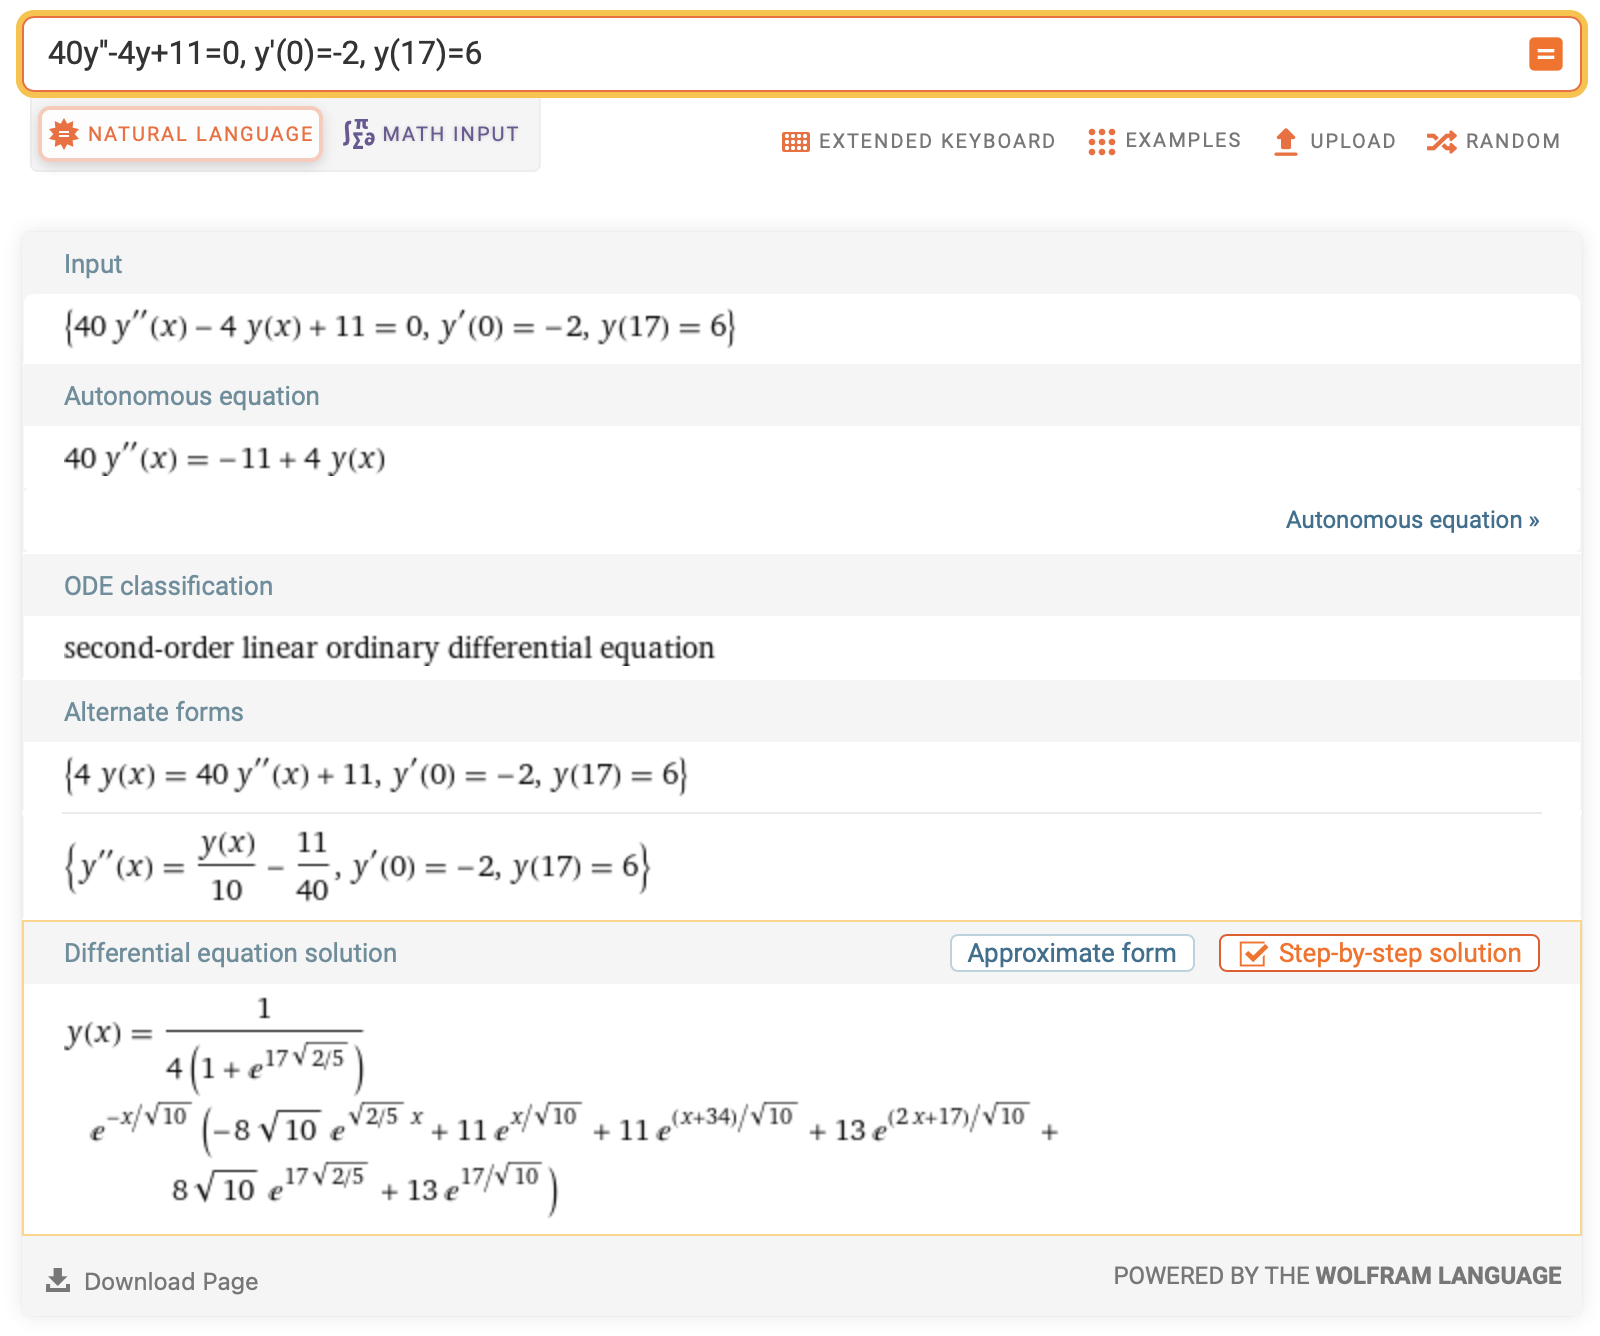
\includegraphics[scale = 0.5]{labs/img/img1}
\end{center}
\caption{Аналитическое решение}
\label{analit}
\end{figure}

Таким образом, получаем:
$$
u(x)=\frac{5}{36}\left(6 x+49 e^{6-(6 x) / 7}-49 e^6+72\right).
$$


\subsection{Получение локальных матрицы жесткости и вектора нагрузок}

Составим локальные матрицу жесткости и вектор нагрузок для уравнения \ref{usl}.

\subsubsection{Линейная функция-формы КЭ}

$$
\mathbf{u}=\begin{bmatrix}
(1-\frac{x}{L}) ; & \frac{x}{L}
\end{bmatrix}
\begin{bmatrix}
u_i \\
u_j
\end{bmatrix}
=\mathbf{N_eU},
$$
где $\mathbf{N_e}$ -- вектор функции формы конечного элемента (в данном случае линейной), его составляющие элементы - глобальные базисные функции, отличные от нуля в пределах этого элемента, $L$ -- длина КЭ.

В соответствии с методом Галеркина для уравнения \ref{usl}:
\begin{equation}\label{lin}
\int_0^L \mathbf{W_e}\left( 7\frac{d^2\mathbf{u}}{dx^2}  +6 \frac{d\mathbf{u}}{dx} -5  \right) d x=0,
\end{equation}
где $\mathbf{W_e=N_e}^T$.

$$\int_0^L \mathbf{W_e}\left(7\frac{d^2\mathbf{u}}{dx^2}  +6 \frac{du}{dx} -5  \right) d x= 7\int_0^L \mathbf{W_e} \frac{d^2 \mathbf{u}}{dx^2} dx   +6  \int_0^L \mathbf{W_e}\frac{d\mathbf{u}}{dx} d x  -5  \int_0^L \mathbf{W_e} d x=0$$

Распишем каждое слагаемое отдельно:
$$
7\int_0^L \mathbf{W_e} \frac{d^2 \mathbf{u}}{dx^2} dx=7\int_0^L
	\begin{bmatrix}
	(1-\frac{x}{L}) \\
	\frac{x}{L}
	\end{bmatrix}
\frac{d^2 \mathbf{u}}{dx^2} dx =
7
	\begin{bmatrix}
	(1-\frac{x}{L}) \\
	\frac{x}{L}
	\end{bmatrix}
\frac{d\mathbf{u}}{dx} |_0^L -
$$
$$
  -7  \int_0^L
\frac{d}{dx}
	\begin{bmatrix}
	(1-\frac{x}{L}) \\
	\frac{x}{L}
	\end{bmatrix}
\frac{d}{dx}
	\begin{bmatrix}
	(1-\frac{x}{L}); & \frac{x}{L}
	\end{bmatrix}
	\begin{bmatrix}
	u_i \\
	u_j
	\end{bmatrix}
=
	\begin{bmatrix}
	  -7 \frac{d\mathbf{u}}{dx}|_i \\
7\frac{d\mathbf{u}}{dx}|_j
	\end{bmatrix}   -7 
\begin{bmatrix}
\frac{1}{L}, & -\frac{1}{L} \\
-\frac{1}{L}, & \frac{1}{L}
\end{bmatrix}
\begin{bmatrix}
u_i \\
u_j
\end{bmatrix}
$$

$$
  +6 \int_0^L \mathbf{W_e} \frac{d \mathbf{u}}{dx} dx=  +6 \int_0^L
	\begin{bmatrix}
	(1-\frac{x}{L}) \\
	\frac{x}{L}
	\end{bmatrix}
\frac{d \mathbf{u}}{dx}
	\begin{bmatrix}
	u_i \\
	u_j
	\end{bmatrix}
dx
=
$$
$$
=
  \frac{6}{L} 
\int_0^L
\begin{bmatrix}
	(1-\frac{x}{L}) & (-1+\frac{x}{L})\\
	-\frac{x}{L} & \frac{x}{L}
\end{bmatrix}
\begin{bmatrix}
	u_i \\
	u_j
\end{bmatrix}
=
  6 
\begin{bmatrix}
-\frac{1}{2}, & \frac{1}{2} \\
-\frac{1}{2}, & \frac{1}{2}
\end{bmatrix}
\begin{bmatrix}
u_i \\
u_j
\end{bmatrix}
$$

$$-5\int_0^L \mathbf{W_e} d x= -5
\begin{bmatrix}
	\frac{L}{2} \\
	\frac{L}{2}
\end{bmatrix}
$$

Таким образом, для уравнения \ref{lin}, при использовании линейной функции-формы,  получаем (матмодель линейного КЭ):

$$
\begin{bmatrix}
	7\frac{1}{L}   +6  \frac{1}{2}, &   -7 \frac{1}{L}   -6  \frac{1}{2} \\
	  -7  \frac{1}{L}  +6  \frac{1}{2}, &  7\frac{1}{L}   -6  \frac{1}{2}
\end{bmatrix}
\begin{bmatrix}
	u_i \\
	u_j
\end{bmatrix}=
\begin{bmatrix}
	  -7 \frac{du}{dx}|_i  -5   \frac{L}{2}\\
	7\frac{du}{dx}|_j  -5   \frac{L}{2}
\end{bmatrix}
$$


\subsubsection{Кубическая функция-формы КЭ}
$$
\mathbf{u}=\begin{bmatrix}
-\frac{9x^3}{2L^3}+\frac{18x^2}{2L^2}-\frac{11x}{2L} + 1;
\frac{27x^3}{2L^3}-\frac{45x^2}{2L^2}+\frac{9x}{L};
-\frac{27x^3}{2L^3}+\frac{36x^2}{2L^2}-\frac{9x}{2L};
\frac{9x^3}{2L^3}-\frac{9x^2}{2L^2}-\frac{x}{L};
\end{bmatrix}
\begin{bmatrix}
u_i \\
u_j\\
u_k\\
u_l
\end{bmatrix}
=\mathbf{N_eU},
$$

Как и для линейной функции-формы применим метод Галеркина (см. уравнение \ref{lin}) и рассмотрим каждое слагаемое отдельно.

$$7 \int_0^L \mathbf{W_e} \frac{d^2 \mathbf{u}}{dx^2} dx
=
7\int_0^L
\begin{bmatrix}
	-\frac{9x^3}{2L^3}&+&\frac{18x^2}{2L^2}&-&\frac{11x}{2L} &+& 1\\
	\frac{27x^3}{2L^3}&-&\frac{45x^2}{2L^2}&+&\frac{9x}{L}&&\\
	-\frac{27x^3}{2L^3}&+&\frac{36x^2}{2L^2}&-&\frac{9x}{2L}&&\\
	\frac{9x^3}{2L^3}&-&\frac{9x^2}{2L^2}&-&\frac{x}{L}&&
\end{bmatrix}
\frac{d^2 \mathbf{u}}{dx^2} dx
=
$$
$$
=
7
\begin{bmatrix}
	-\frac{9x^3}{2L^3}&+&\frac{18x^2}{2L^2}&-&\frac{11x}{2L} &+& 1\\
	\frac{27x^3}{2L^3}&-&\frac{45x^2}{2L^2}&+&\frac{9x}{L}&&\\
	-\frac{27x^3}{2L^3}&+&\frac{36x^2}{2L^2}&-&\frac{9x}{2L}&&\\
	\frac{9x^3}{2L^3}&-&\frac{9x^2}{2L^2}&-&\frac{x}{L}&&
\end{bmatrix}
\frac{d\mathbf{u}}{dx} |_0^L
  -7  \int_0^L \frac{d}{dx}
\begin{bmatrix}
	-\frac{9x^3}{2L^3}&+&\frac{18x^2}{2L^2}&-&\frac{11x}{2L} &+& 1\\
	\frac{27x^3}{2L^3}&-&\frac{45x^2}{2L^2}&+&\frac{9x}{L}&&\\
	-\frac{27x^3}{2L^3}&+&\frac{36x^2}{2L^2}&-&\frac{9x}{2L}&&\\
	\frac{9x^3}{2L^3}&-&\frac{9x^2}{2L^2}&-&\frac{x}{L}&&
\end{bmatrix}
\frac{d}{dx} \mathbf{u}
=$$
$$
=
\begin{bmatrix}
	  -7 \frac{d\mathbf{u}}{dx}|_i \\
	0\\
	0\\
7\frac{d\mathbf{u}}{dx}|_l
\end{bmatrix}
  -7 
\begin{bmatrix}
\begin{array}{rrrr}
	\frac{37}{10L} & -\frac{189}{40} & \frac{27}{20L} & -\frac{13}{40L}\\
	-\frac{189}{40} & \frac{54}{5L} & -\frac{297}{40L} & \frac{27}{20L}\\
	\frac{27}{20L} &  -\frac{297}{40L} & \frac{54}{5L} & -\frac{189}{40}\\
	-\frac{13}{40L} & \frac{27}{20L} & -\frac{189}{40} & \frac{37}{10L}
\end{array}
\end{bmatrix}
\begin{bmatrix}
u_i \\
u_j \\
u_k\\
u_l
\end{bmatrix}
$$

$$
  +6  \int_0^L \mathbf{W_e} \frac{d \mathbf{u}}{dx} dx
=
  +6 \int_0^L
\begin{bmatrix}
  -\frac{9x^3}{2L^3}&+&\frac{18x^2}{2L^2}&-&\frac{11x}{2L} &+& 1\\
  \frac{27x^3}{2L^3}&-&\frac{45x^2}{2L^2}&+&\frac{9x}{L}&&\\
  -\frac{27x^3}{2L^3}&+&\frac{36x^2}{2L^2}&-&\frac{9x}{2L}&&\\
  \frac{9x^3}{2L^3}&-&\frac{9x^2}{2L^2}&-&\frac{x}{L}&&
\end{bmatrix}
\frac{d \mathbf{u}}{dx} dx
=
$$
$$
=
  +6 
\begin{bmatrix}
\begin{array}{rrrr}
	-\frac{1}{2} & \frac{57}{80} & -\frac{3}{10} & \frac{7}{80}\\
	-\frac{57}{80} & 0 & \frac{81}{80} & -\frac{3}{10} \\
	\frac{3}{10} & -\frac{81}{80} & 0 & -\frac{3}{10}\\
	-\frac{7}{80} & \frac{3}{10} & -\frac{57}{80} & \frac{1}{2}
\end{array}
\end{bmatrix}
\begin{bmatrix}
	u_i \\
	u_j \\
	u_k\\
	u_l
\end{bmatrix}
$$

$$
-5 \int_0^L \mathbf{W_e} d x
=
-5
\begin{bmatrix}
	\frac{L}{8} \\
	\frac{3L}{8}\\
	\frac{3L}{8}\\
	\frac{L}{8}
\end{bmatrix}
$$

\newpage
Таким образом, для уравнения \ref{lin}, при использовании кубической функции-формы,  получаем:

\begin{align}\label{cub}
\begin{bmatrix}7\frac{37}{10L}  +6 \frac{1}{2} &   -7 \frac{189}{40L}  -6 \frac{57}{80} & 7\frac{27}{20L}  +6 \frac{3}{10} &   -7 \frac{13}{40L}   -6  \frac{7}{80}\\
	  -7 \frac{189}{40L}   +6 \frac{57}{80} & 7\frac{54}{5L}+0 &   -7 \frac{297}{40L}  -6 \frac{81}{80} & 7\frac{27}{20L}   +6 \frac{3}{10} \\
	7\frac{27}{20L}   -6  \frac{3}{10} &   -7 \frac{297}{40L}  +6 \frac{81}{80} & 7\frac{54}{5L}+0 &   -7 \frac{189}{40L}   -6 \frac{57}{80} \\
	  -7 \frac{13}{40L}   +6 \frac{7}{80} & 7\frac{27}{20L}  -6 \frac{3}{10} &   -7 \frac{189}{40L}  -6 \frac{57}{80} & 7\frac{37}{10L}   -6 \frac{1}{2}
\end{bmatrix}
\begin{bmatrix}
	u_i \\
	u_j \\
	u_k\\
	u_l
\end{bmatrix}
=
\begin{bmatrix}
    -5\frac{L}{8}   -7  \frac{du}{dx}|_i \\
	-5\frac{3L}{8}\\
	-5\frac{3L}{8}\\
	-5\frac{L}{8}   +7  \frac{du}{dx}|_l
\end{bmatrix}
\end{align}

Локальные матрица жесткости и вектор нагрузок могут быть представлены в виде:
$$ \begin{bmatrix}
a_{11}     &  a_{12}  &  a_{13} &  a_{14}\\
a_{21}     &  a_{22}  &  a_{23} &  a_{24}\\
a_{31}     &  a_{32}  &  a_{33} &  a_{34}\\
a_{41}     &  a_{42}  & a_{43}  &  a_{44}
\end{bmatrix}
\begin{bmatrix}
u_i \\
u_j \\
u_k\\
u_l
\end{bmatrix} =
\begin{bmatrix}
b_1 - 2 \frac{du}{dx}|_i \\
b_2\\
b_3\\
b_4 + 2 \frac{du}{dx}|_l
\end{bmatrix}$$

Выполним матричные преобразования.
$$ \begin{bmatrix}
a_{11} -\frac{a_{12}}{a_{22}}{a_{21}}    &  a_{12} -\frac{a_{12}}{a_{22}}{a_{22}}  &  a_{13} -\frac{a_{12}}{a_{22}}{a_{23}} &  a_{14}-\frac{a_{12}}{a_{22}}{a_{24}}\\
a_{21}     &  a_{22}  &  a_{23} &  a_{24}\\
a_{31} -\frac{a_{32}}{a_{22}}{a_{21}}   &  a_{32}-\frac{a_{32}}{a_{22}}{a_{22}}  &  a_{33}-\frac{a_{32}}{a_{22}}{a_{23}} &  a_{34}-\frac{a_{32}}{a_{22}}{a_{24}}\\
a_{41}  -\frac{a_{42}}{a_{22}}{a_{21}}   &  a_{42} -\frac{a_{42}}{a_{22}}{a_{22}}  & a_{43}-\frac{a_{42}}{a_{22}}{a_{23}}  &  a_{44}-\frac{a_{42}}{a_{22}}{a_{24}}
\end{bmatrix}
\begin{bmatrix}
u_i \\
u_j \\
u_k\\
u_l
\end{bmatrix} =
\begin{bmatrix}
b_1-\frac{a_{12}}{a_{22}}{b_{2}}   -7  \frac{du}{dx}|_i \\
b_2\\
b_3 - \frac{a_{32}}{a_{22}}{b_{2}}\\
b_4 - \frac{a_{42}}{a_{22}}{b_{2}}   +7  \frac{du}{dx}|_l
\end{bmatrix}$$

% ---------------------------второе

$$ \begin{bmatrix}
a_{11}'-\frac{a_{13}'}{a_{33}'}a_{31}'   &  0 -\frac{a_{13}'}{a_{33}'}0  &  a_{13}'--\frac{a_{13}'}{a_{33}'}a_{33}' &  a_{14}'-\frac{a_{13}'}{a_{33}'}a_{34}'\\
a_{21}' -\frac{a_{23}'}{a_{33}'}a_{31}'    &  a_{22}' -\frac{a_{23}'}{a_{33}'}0  &  a_{23}' -\frac{a_{23}'}{a_{33}'}a_{33}' &  a_{24}' -\frac{a_{23}'}{a_{33}'}a_{34}'\\
a_{31}'     &  0  &  a_{33}' &  a_{34}'\\
a_{41}'  -\frac{a_{43}'}{a_{33}'}a_{31}'    &  0-\frac{a_{43}'}{a_{33}'}0  & a_{43}'-\frac{a_{43}'}{a_{33}'}a_{33}'  &  a_{44}'-\frac{a_{43}'}{a_{33}'}a_{34}'
\end{bmatrix}
\begin{bmatrix}
u_i \\
u_j \\
u_k\\
u_l
\end{bmatrix} =
\begin{bmatrix}
b_1'-\frac{a_{13}'}{a_{33}'}b_{3}'   -7  \frac{du}{dx}|_i \\
b_2'-\frac{a_{23}'}{a_{33}'}b_{3}'\\
b_3'\\
b_4' -\frac{a_{43}'}{a_{33}'}b_{3}'   +7  \frac{du}{dx}|_l
\end{bmatrix}$$

Итого получаем:

$$ \begin{bmatrix}
a_{11}''     &  0  & 0  &  a_{14}''\\
a_{21}''     &  a_{22}''  & 0  &  a_{24}''\\
a_{31}''     &  0  &  a_{33}'' &  a_{34}''\\
a_{41}''    &  0  & 0  &  a_{44}''
\end{bmatrix}
\begin{bmatrix}
u_i \\
u_j \\
u_k\\
u_l
\end{bmatrix} =
\begin{bmatrix}
b_1'' ^{}   -7  \frac{du}{dx}|_i \\
b_2''\\
b_3''\\
b_4''   +7  \frac{du}{dx}|_l
\end{bmatrix}$$

Для упрощения расчетов преобразуем систему выше, исключив внутренние узлы.


Таким образом, при использовании кубической функции-формы,  получаем:
$$ \begin{bmatrix}
a_{11}''     &   a_{14}''\\
a_{41}''     &    a_{44}''
\end{bmatrix}
\begin{bmatrix}
u_i \\
u_l
\end{bmatrix} =
\begin{bmatrix}
b_{1}'' ^{}   -7  \frac{du}{dx}|_i \\
b_4''   +7  \frac{du}{dx}|_l
\end{bmatrix}$$

~\\
~\\
% %~\\


%-------------------------------------------------
\subsection{Получение глобальных матрицы жесткости и вектора нагрузок}

Проведем процедуры ансамблирования и учет граничных условий для формирования итоговой математической модели.

\subsubsection{Ансамблирование}

Пусть локальные матрица жесткости и вектор неизвестных заданы следующим образом

$$
\begin{bmatrix}
a_{11}     &   a_{12}\\
a_{21}     &    a_{22}
\end{bmatrix}
\begin{bmatrix}
u_i \\
u_j
\end{bmatrix} =
\begin{bmatrix}
b_1   -7  \frac{du}{dx}|_i \\
b_2   +7  \frac{du}{dx}|_l
\end{bmatrix},$$

тогда, при разбитие области на $n$ КЭ, глобальная матрица жесткости  будет иметь размерность $(n+1)\cdot(n+1)$:

$$ \begin{bmatrix}
a_{11}^1     &   a_{12}^1         &   0 & \cdots & 0 & 0 & 0  & 0\\
a_{21}^1     &    a_{22}^1+a_{11}^2 & a_{12}^2  & 0 & \cdots & 0 & 0  & 0\\
0     &    a_{21}^2 & a_{22}^2+a_{11}^3  &  a_{12}^3  & 0 & \cdots & 0  & 0\\
0     &    0  & a_{21}^3  & a_{22}^3+ \cdots  &  & &   & 0\\
\vdots & \vdots & \vdots & \vdots &  &  &   & \vdots\\
0 & 0 & 0 & 0 &  0 & 0 & \cdots+a_{11}^n  & a_{12}^n\\
0 & 0 & 0 & 0 &  0 & 0 & a_{21}^n  & a_{22}^n
\end{bmatrix}
\begin{bmatrix}
u_0 \\
u_1 \\
u_2\\
u_3\\
\vdots\\
u_{n-1}\\
u_n
\end{bmatrix} =
\begin{bmatrix}
b_1^1   -7  \frac{du}{dx}|_0 \\
b_2^1+b_1^2\\
b_2^2+b_1^3\\
b_2^3+b_1^4\\
\vdots\\
b_2^{n-1}+b_1^n\\
b_2^n   +7  \frac{du}{dx}|_L
\end{bmatrix}
$$

\subsubsection{Учет граничных условий}

Применим граничные условия первого (см. \ref{1_gu}) и  второго  рода (см. \ref{2_gu}) к выведенной выше системе.

$$
\begin{bmatrix}
1 & 0 &   0 & \cdots & 0 & 0 & 0  & 0\\
a_{21}^1 & a_{22}^1+a_{11}^2 & a_{12}^2  & 0 & \cdots & 0 & 0  & 0\\
0 & a_{21}^2 & a_{22}^2+a_{11}^3  &  a_{12}^3  & 0 & \cdots & 0  & 0\\
0 & 0 & a_{21}^3  & a_{22}^3+ \cdots  &  & &   & 0\\
\vdots & \vdots & \vdots & \vdots &  &  &   & \vdots\\
0 & 0 & 0 & 0 &  0 & 0 & \cdots+a_{11}^n  & a_{12}^n\\
0 & 0 & 0 & 0 &  0 & 0 & a_{21}^n  & a_{22}^n
\end{bmatrix}
\begin{bmatrix}
u_0 \\
u_1 \\
u_2\\
u_3\\
\vdots\\
u_{n-1}\\
u_n
\end{bmatrix} =
\begin{bmatrix}
 10   \\
b_2^1+b_1^2\\
b_2^2+b_1^3\\
b_2^3+b_1^4\\
\vdots\\
b_2^{n-1}+b_1^n\\
 b_2^n   +7  \cdot -5   \\
\end{bmatrix}
$$

\subsection{Анализ результатов}

Проведем сравнение результатов согласно заданию.

\subsubsection{Линейная функция-формы}


На рисунках \ref{l_20}, \ref{l_40} представлены графики полученные с помощью МКЭ (линейная функция-формы).

\begin{figure}[!h]
    \centering
    \begin{minipage}{0.5\textwidth}
        \centering
        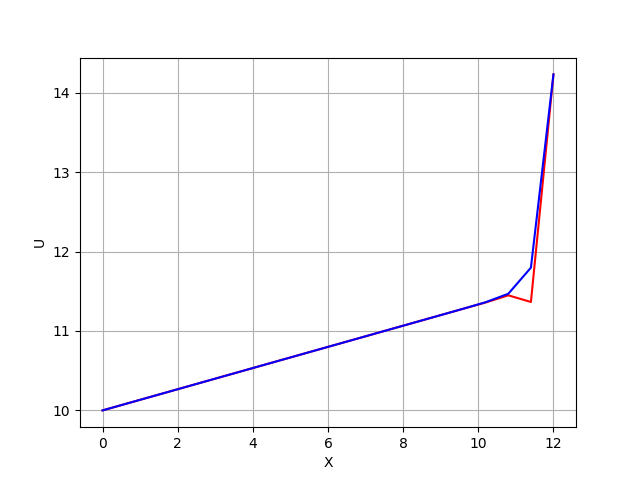
\includegraphics[width=1\textwidth]{labs/img/lin/20.png} % первое изображениие
        \caption{Результат работы программы для 20 КЭ}
        \label{l_20}
    \end{minipage}\hfill
    \begin{minipage}{0.5\textwidth}
        \centering
        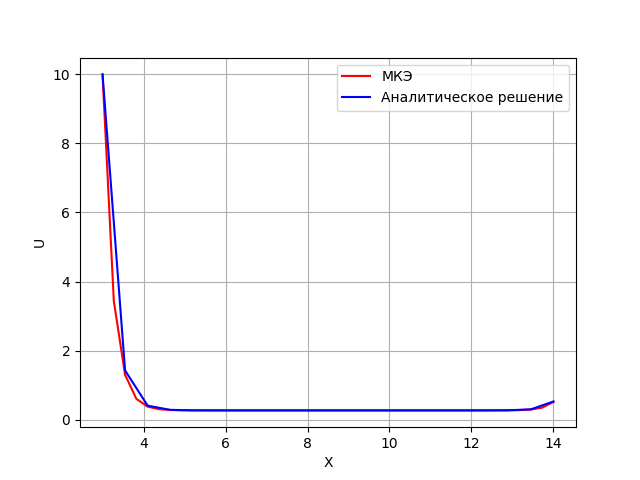
\includegraphics[width=1\textwidth]{labs/img/lin/40.png} % второе изображение
        \caption{Результат работы программы для 40 КЭ}
        \label{l_40}
    \end{minipage}
\end{figure}

\begin{table}[H]
\centering
\begin{tabular}{|c|c|c|c|}
\hline
X & Аналитическое & МКЭ-    & Абсолютная \\
  & решение       & решение & погрешность \\
\hline
\input{labs/text/tab/lin_20.txt} \\
\hline
\end{tabular}
\caption{20 линейных КЭ}
\label{table:lin_20}
\end{table}

\begin{table}[H]
\centering
\begin{tabular}{|c|c|c|c|}
\hline
X & Аналитическое & МКЭ-    & Абсолютная \\
  & решение       & решение & погрешность \\
\hline
\input{labs/text/tab/lin_40.txt} \\
\hline
\end{tabular}
\caption{40 линейных КЭ}
\label{table:lin_40}
\end{table}

Максимальная абсолютная погрешность \input{labs/text/pgr/lin_20.txt} и \input{labs/text/pgr/lin_40.txt} соответственно.

\subsubsection{Кубическая функция-формы}

На рисунках \ref{c_20}, \ref{c_40} представлены графики полученные с помощью МКЭ (кубическая функция-формы).

\begin{figure}[!h]
    \centering
    \begin{minipage}{0.5\textwidth}
        \centering
        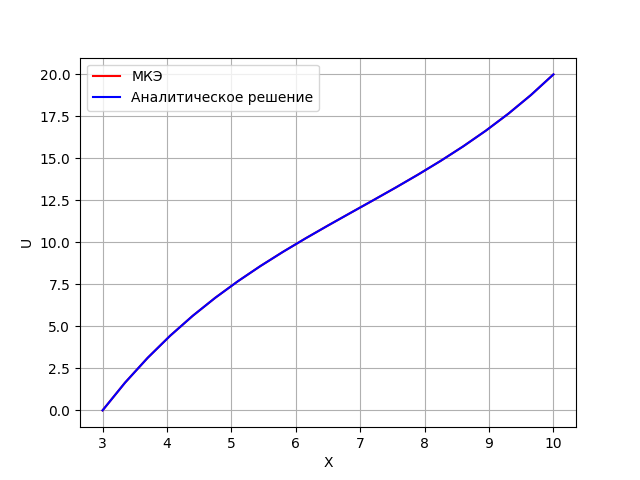
\includegraphics[width=1\textwidth]{labs/img/cub/20.png} % первое изображениие
        \caption{Результат работы программы для 20 КЭ}
        \label{c_20}
    \end{minipage}\hfill
    \begin{minipage}{0.5\textwidth}
        \centering
        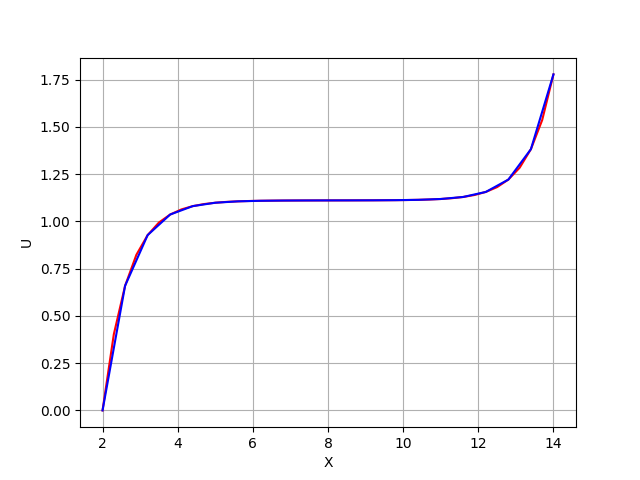
\includegraphics[width=1\textwidth]{labs/img/cub/40.png} % второе изображение
        \caption{Результат работы программы для 40 КЭ}
        \label{c_40}
    \end{minipage}
\end{figure}

\begin{table}[H]
\centering
\begin{tabular}{|c|c|c|c|}
\hline
X & Аналитическое & МКЭ-    & Абсолютная \\
  & решение       & решение & погрешность \\
\hline
\input{labs/text/tab/cub_20.txt} \\
\hline
\end{tabular}
\caption{20 кубических КЭ}
\label{table:lin_20}
\end{table}

\begin{table}[H]
\centering
\begin{tabular}{|c|c|c|c|}
\hline
X & Аналитическое & МКЭ-    & Абсолютная \\
  & решение       & решение & погрешность \\
\hline
\input{labs/text/tab/cub_40.txt} \\
\hline
\end{tabular}
\caption{40 кубических КЭ}
\label{table:lin_40}
\end{table}

Максимальная абсолютная погрешность \input{labs/text/pgr/cub_20.txt} и \input{labs/text/pgr/cub_40.txt} соответственно.


\subsubsection{Нахождение количества линейных КЭ, обеспечивающих ту же точность, что и 20 кубических}

Так как очевидно, что при увлечении числа КЭ точность растет, найдем искомое следуя алгоритму, представленному на рисунке \ref{alg}.

\begin{figure}[H]
\centerline{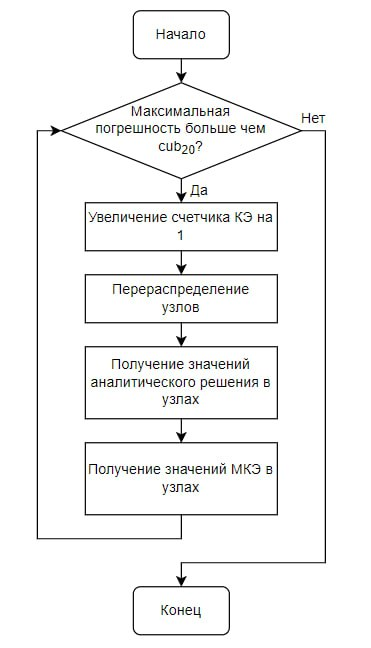
\includegraphics[scale = 0.65]{labs/img/img2.jpg}}
\caption{Алгоритм нахождения количества КЭ, заданную точность ($cub_{20} = \input{labs/text/pgr/cub_20.txt}$)}
\label{alg}
\end{figure}

Реализовав данный алгоритм с начальным количеством КЭ=20 и увеличивая счетчик всегда на 1 получаем необходимое количество КЭ, равное \input{labs/text/pogr.txt}.

\subsection{Код}

\begin{lstlisting}[language=c++, label=prog,caption={\textit{Реализация МКЭ}}]

#include <iostream>
#include <vector>
#include <cmath>

//#define OSN 
//#define TABLE
//#define CUBE

constexpr double EPS = 1e-16,CUB= 0.0001195516;
double EPS = 1e-16;
double X_BEGIN = 0.0;
double X_END = 7.0;
size_t ELEMS_NUM = ;
double L = (X_END - X_BEGIN) / ELEMS_NUM;

constexpr double a = 7.0, B = 6.0, C = 0.0, D = -5.0, usl_left = 10.0, usl_right = -5.0; // au"+Bu'+Cu+D=0

std::vector<double> solve_with_gauss(std::vector<std::vector<double>>& A, std::vector<double>& b){
    size_t row_size = A.size();
    size_t col_size = A.back().size();
    // Прямой ход Гаусса
    double pivot = 0.0;
    for (size_t i = 0; i < row_size; i++) {
        for (size_t j = i + 1; j < col_size; j++) {
            if (std::abs(A.at(j).at(i)) < EPS) {
                continue;
            }
            pivot = A.at(j).at(i) / A.at(i).at(i);
            b.at(j) -= pivot * b.at(i);
            for (size_t k = 0; k < row_size; k++) {
                A.at(j).at(k) -= pivot * A.at(i).at(k) ;
            }
        }
    }
    // Обратный ход Гаусса
    std::vector<double> x(row_size);
    for (int i = row_size - 1.0; i >= 0; i--) {
        x.at(i) = b.at(i);
        for (size_t j = i + 1; j < row_size; j++) {
            x.at(i) -= x.at(j) * A.at(i).at(j);
        }
        x.at(i) /= A.at(i).at(i);
    }
    return x;
}

double analytical_solution(double x) {
    double rez = 5. / 36. * (6. * x + 49. * exp(6. - (6. * x) / 7.) - 49. * exp(6.) + 72.);
    return rez;
}

std::vector<double> build_analytical_solution(std::vector<double>& x_vec) {
    size_t x_vec_size = x_vec.size();
    std::vector<double> y_vec = std::vector<double>(x_vec_size);
    for (size_t i = 0; i < x_vec_size; i++) {
        y_vec.at(i) = analytical_solution(x_vec.at(i));
    }
    return y_vec;
}

std::vector<double> build_linear_solution(size_t elems_num) {
    double L = (X_END - X_BEGIN) / elems_num;
    size_t size = elems_num + 1;
    std::vector< std::vector<double> > A(size, std::vector<double>(size));
    std::vector<double> b(size);
    
    // Локальная матрица жесткости для линейного КЭ
    std::vector< std::vector<double> > local_matrix = {
        { a/L - C * L/3.0 + B*1.0/2.0, -a/L - C * L/6.0 - B*1.0/2.0},
        { -a/L - C * L/6.0 + B*1.0/2.0, a/L - C*L/3.0 - B*1.0/2.0},
    };
    
    // Ансамблирование и получение глобальной матрицы жесткости для линейного КЭ
    for (size_t i = 0; i < elems_num; i++) {
        for (size_t j = 0; j < 2; j++) {
            for (size_t k = 0; k < 2; k++) {
                A.at(i + j).at(i + k) += local_matrix.at(j).at(k);
            }
        }
    }
    
        for (size_t i = 0; i < size ; i++) {
        b.at(i) = D * L;
    }
    
    // Учет ГУ 
    b.at(0) = usl_left;
    A.at(0).at(0) = 1;
    A.at(0).at(1) = 0;
    
    b.at(size - 1) =  D * L /2. + a*usl_right;
    
    // Решение полученной СЛАУ методом Гаусса
    std::vector<double> res = solve_with_gauss(A, b);
    return res;
}

std::vector<double> build_cube_solution(size_t elems_num) {
    double L = (X_END - X_BEGIN) / elems_num;
    size_t size = elems_num + 1;
    std::vector< std::vector<double> > A(size,std::vector<double>(size));
    std::vector<double> b(size);
    
    // Локальная матрица жесткости для кубического КЭ
       std::vector< std::vector<double> > local_matrix = {

        {  a*37.0/(10.0*L) - C*8*L/105.0 +B*1.0/2.0,    -a*189.0/(40.0*L) - C*33*L/560.0 - B*57/80.0, a*27.0/(20.0*L) + C*3*L/140.0 + B*3.0/10.0, -a*13.0/(40.0*L) -  C*19.0*L/1680.0 - B*7/80.0},
        { -a*189.0/(40.0*L) - C*33*L/560.0 + B*57/80.0,  a*54.0/(5.0*L)-C*27*L/70.0,                  -a*297.0/(40*L) + C*27*L/560.0 - B*81.0/80.0,    a*27.0/(20.0*L) +  C*3*L/140.0 + B*3.0/10.0},
        {  a*27.0/(20.0*L) + C*3*L/140.0 - B*3.0/10.0,  -a*297.0/(40.0*L) + C*27*L/560.0 + B*81.0/80.0,  a*54.0/(5.0*L) - C*27*L/70.0,                -a*189.0/(40.0*L) - C*33*L/560.0 - B*57/80.0},
        { -a*13.0/(40.0*L) - C*19.0*L/1680.0 + B*7/80.0,   a*27.0/(20.0*L) + C*3*L/140.0 - B*3.0/10.0 , -a*189.0/(40.0*L) - C*33*L/560.0 + B*57/80.0,      a*37.0/(10.0*L) - C*8*L/105.0 - B*1.0/2.0}
        
   };
    
    // Локальный вектор нагрузок (дополнительные слагаемые для первого и последнего элементов учитываются далее)
    std::vector<double> local_b = { D * L / 8.0,
                                    D*3.0 * L / 8.0,
                                    D*3.0 * L / 8.0, 
                                    D * L / 8.0 };

    
    // Производим матричные преобразования для обнуления элементов локальной матрицы жесткости, относящихся к внутренним узлам
    for (size_t i = 1; i < 3; i++) {
        for (size_t j = 0; j < 4; j++) {
            if (std::fabs(local_matrix.at(j).at(i)) > EPS && i != j) {
                double  val = local_matrix.at(j).at(i) /local_matrix.at(i).at(i);
                local_b.at(j) -= val * local_b.at(i);
                for (size_t k = 0; k < 4; k++) {
                    local_matrix.at(j).at(k) -= val *local_matrix.at(i).at(k);
                }
            }
            continue;
        }
    }
    
    
    // Исключаем внутренние узлы из рассмотрения
    std::vector< std::vector<double> >  local_matrix_mod  = { { local_matrix.at(0).at(0), local_matrix.at(0).at(3) },
                                                             { local_matrix.at(3).at(0), local_matrix.at(3).at(3) } };
    std::vector<double> local_b_mod = { local_b.at(0), 
                                        local_b.at(3)};
    
    // Ансамблирование и получение глобальной матрицы жесткости для кубического КЭ
    for (size_t i = 0; i < elems_num; i++) {
        for (size_t j = 0; j < 2; j++) {
            for (size_t k = 0; k < 2; k++) {
                A.at(i + j).at(i + k) += local_matrix_mod.at(j).at(k);
            }
        }
    }
        for (size_t i = 0; i < elems_num; i++) {
        b.at(i) += local_b_mod.at(0);
        b.at(i+1) += local_b_mod.at(1);
    }
    // Учет ГУ
    b.at(0) = usl_left;
    A.at(0).at(0) = 1;
    A.at(0).at(1) = 0;
    
    b.at(size - 1) =  local_b_mod.at(1) + a * usl_right;
    
    // Решение полученной СЛАУ методом Гаусса
    std::vector<double> res = solve_with_gauss(A, b);
    return res;
}

double calc_abs_error(const std::vector<double>& y_real, const std::vector<double>& y) {
    double max_err = 0.0;
    for (size_t i = 0; i < y_real.size(); i++) {
        double err = std::fabs(y_real.at(i) - y.at(i));
        if (err > max_err) {
            max_err = err;
        }
    }
    return max_err;
}

int main() {
#ifdef OSN

    std::vector<double> x(ELEMS_NUM + 1);
    for (size_t i = 0; i < x.size(); i++) {
        x.at(i) = X_BEGIN + i * L;
    }
    size_t x_size = x.size();
    

#ifdef CUBE
    std::vector<double> y = build_cube_solution(ELEMS_NUM);
#else
    std::vector<double> y = build_linear_solution(ELEMS_NUM);
#endif
    std::vector<double> y_real = build_analytical_solution(x);
     
#ifdef TABLE
    for (size_t i = 0; i < x.size(); i++) {
        std::cout<<x.at(i)<<" & "<<y_real.at(i)<<" &"<<y.at(i)<<" &"<<std::fabs(y_real.at(i) - y.at(i))<<"\\\\"<<std::endl;
    }
#endif    

    FILE* gp = popen("gnuplot -persist", "w");
    fprintf(gp, "$predict << EOD\n");
    for (size_t i = 0; i < x_size; i++) {
        fprintf(gp, "%lf %lf\n", x.at(i), y.at(i));
    }
    fprintf(gp, "EOD\n");
    fprintf(gp, "$real << EOD\n");
    for (size_t i = 0; i < x_size; i++) {
        fprintf(gp, "%lf %lf\n", x.at(i), y_real.at(i));
    }
    fprintf(gp, "EOD\n");
    fprintf(gp, "set grid\n");
     fprintf(gp, "plot '$predict' using 1:2 with lp lc '#ba55d3' lw 1.5 pt 7 ps 0.5 title 'МКЭ-решение (%zu КЭ)'," "'$real' using 1:2 with lines lc rgb '#afdafc' lt 1 lw 2 title 'аналитическое решение (%zu КЭ)',\n", ELEMS_NUM, ELEMS_NUM);
     printf("Абсолютная погрешность: %e\n", calc_abs_error(y_real, y));

     
    //нахождение количества линейных КЭ
#else
    int N=20,n=10000;
    double err=10;
    FILE* gp = popen("gnuplot -persist", "w");
    fprintf(gp, "$predict << EOD\n");
    while (err>CUB && n<=19000){
        
        double L = (X_END - X_BEGIN) / N;
        std::vector<double> x(N + 1);
        for (size_t i = 0; i < x.size(); i++) {
            x.at(i) = X_BEGIN + i * L;
        }
        
        std::vector<double> y_r(N + 1);
        std::vector<double> y_s(N + 1);
        
        y_s = build_linear_solution(N);
        y_r = build_analytical_solution(x);
        
        err=calc_abs_error(y_r, y_s);
        
        fprintf(gp, "%d %e\n", N, err);
        printf("Абсолютная погрешность: %e   количество КЭ: %d\n", calc_abs_error(y_r, y_s), N);
        N+=1;
        n+=1;
    }
    
    fprintf(gp, "EOD\n");
    fprintf(gp, "set grid\n");
    fprintf(gp, "set logscale y 2\n");
    fprintf(gp, "plot '$predict' using 1:2 with lp lc '#cd853f' lw 1.5 pt 7 ps 0.5 title 'Абсолютная погрешность',\n" );
    std::cout<<"Количество линейных КЭ "<<N-1<<std::endl;
    printf("Абсолютная погрешность: %e\n", err);

#endif 
    return 0;
}

\end{lstlisting}
%-------------------------------------------------
\subsection{Вывод}

В ходе выполнения лабораторной работы был реализован МКЭ для различных функций форм, а также найдено количество линейных КЭ обеспечивающих точность 20ти кубических КЭ.

% --------------------------------------
% Атрибуты задачи
\labattributes{}{}{}{}{студент группы \EduGroup, \Author}{\Year, \Semestr}
%--------------

%   +7 
%   -7 

%   +6 
%   -6 

%  -5  
%  +5  
%----------------------------------------------------------
%\bibliography{bibliographyVariantNM}
%----------------------------------------------------------
\end{document}
%----------------------------------------------------------



